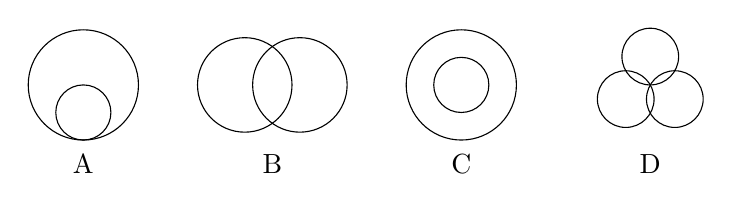
\begin{tikzpicture}\begin{scope}\draw(0,0)circle(.7);\draw(0,-.35)circle(.35);\node at(0,-1){A};\end{scope}\begin{scope}[shift={(2.4,0)}]\draw(-.35,0)circle(.6);\draw(.35,0)circle(.6);\node at(0,-1){B};\end{scope}\begin{scope}[shift={(4.8,0)}]\draw(0,0)circle(.7);\draw(0,0)circle(.35);\node at(0,-1){C};\end{scope}\begin{scope}[shift={(7.2,0)}]\foreach \a in {90,210,330}{\draw(\a:.36)circle(.36);}\node at(0,-1){D};\end{scope}\end{tikzpicture}
